\documentclass[10pt]{article}
\usepackage[a4paper,margin=14.5mm,headheight=20pt,headsep=3mm,footskip=19pt]{geometry}
\usepackage{fontspec}
\setmainfont{Palatino}
\setsansfont{Avenir Next}
\setmonofont{Menlo}
\newfontfamily\displayfont{Baskerville}
\usepackage{amsmath,amssymb}
\usepackage{booktabs,tabularx,array,multicol}
\usepackage{tikz}
\usetikzlibrary{positioning,arrows.meta}
\usepackage{pgfplots}
\pgfplotsset{compat=1.18}
\usepackage[most]{tcolorbox}
\tcbuselibrary{skins,breakable}
\usepackage{enumitem}
\usepackage{titlesec}
\usepackage{fancyhdr}
\usepackage{microtype}
\usepackage{float}
\usepackage[hidelinks]{hyperref}

\definecolor{Ink}{HTML}{202A30}
\definecolor{Muted}{HTML}{63737A}
\definecolor{Teal}{HTML}{247A73}
\definecolor{Rust}{HTML}{C25132}
\definecolor{Blue}{HTML}{557A92}
\definecolor{Purple}{HTML}{7968A3}
\definecolor{Gold}{HTML}{C58A2A}
\definecolor{Pale}{HTML}{F1F5F4}
\definecolor{PaleWarm}{HTML}{FBF3EF}
\definecolor{Rule}{HTML}{D9E1DF}

\hypersetup{pdftitle={COMP3314 Group 27 — MDA Face Recognition Final Report},pdfauthor={COMP3314 Group 27},pdfsubject={Paper-proximate reproduction of Multilinear Discriminant Analysis on ORL faces}}
\pagestyle{fancy}
\fancyhf{}
\fancyhead[L]{\sffamily\small\color{Muted}COMP3314 \; / \; GROUP 27}
\fancyhead[R]{\sffamily\small\color{Muted}MDA FACE RECOGNITION}
\fancyfoot[C]{\sffamily\small\color{Muted}\thepage\; / \;4}
\renewcommand{\headrulewidth}{0.45pt}
\renewcommand{\headrule}{\hbox to\headwidth{\color{Rule}\leaders\hrule height \headrulewidth\hfill}}
\setlength{\parindent}{0pt}
\setlength{\parskip}{0.42em}
\setlength{\emergencystretch}{2em}
\setlist[itemize]{leftmargin=1.2em,itemsep=0.15em,topsep=0.15em}
\titleformat{\section}{\sffamily\large\bfseries\color{Teal}}{}{0pt}{}
\titlespacing*{\section}{0pt}{0.55em}{0.25em}
\newtcolorbox{softbox}[1][]{colback=Pale,colframe=Pale,boxrule=0pt,arc=2mm,left=2.4mm,right=2.4mm,top=1.7mm,bottom=1.7mm,#1}
\newtcolorbox{warmbox}[1][]{colback=PaleWarm,colframe=PaleWarm,boxrule=0pt,arc=2mm,left=2.4mm,right=2.4mm,top=1.7mm,bottom=1.7mm,#1}
\newtcolorbox{videobox}{colback=Pale,colframe=Pale,boxrule=0pt,arc=2mm,borderline west={2pt}{0pt}{Teal},left=2.4mm,right=2.4mm,top=1.4mm,bottom=1.4mm}
\tikzset{
  stepbox/.style={draw=Rule,fill=Pale,rounded corners=2mm,align=center,text=Ink,font=\sffamily\small,minimum height=13mm,text width=34mm,inner sep=2mm},
  arrow/.style={-{Stealth[length=2mm]},draw=Muted,line width=0.8pt},
  dot/.style={circle,fill=Teal,draw=none,minimum size=2.5mm,inner sep=0pt}
}
\newcommand{\smallcaps}[1]{{\sffamily\bfseries\color{Teal}\footnotesize #1}}
\newcommand{\pp}{\,\text{pp}}

\begin{document}
\thispagestyle{fancy}

\begin{center}
{\sffamily\bfseries\color{Teal}\small COMP3314 \; | \; GROUP 27 \; | \; FALL 2026}\par
\vspace{2mm}
{\displayfont\fontsize{25}{29}\selectfont\color{Ink}Multilinear Discriminant Analysis\par for Face Recognition}\par
\vspace{1.5mm}
{\sffamily\small\color{Muted}A paper-proximate study on original-resolution ORL faces}\par
\vspace{1mm}
{\sffamily\footnotesize Jad Khiami \; · \; Lai Hing Kwan \; · \; Lam Cheung Lam \; · \; Lan Yuhang}
\end{center}

\begin{softbox}
\smallcaps{Abstract}\par
Yan et al. introduced Multilinear Discriminant Analysis (MDA), which learns identity-discriminating projections while retaining the row and column structure of an image. We implemented the core method on the original 112\,$\times$\,92 ORL faces and compared it with PCA, Fisherfaces, and two MDA variants. In the fixed-setting study, MDA/2-1 led at every gallery size, while MDA/2-2 was highly sensitive to projection-axis normalization. Our full dimension grids remain below the paper's reported best scores and are optimistic because probe scores selected the dimensions. Since several paper settings are unspecified, we report this as a paper-proximate reproduction, document our choices, and preserve the complete direct-run data. A corrected cached implementation is now the default for future sweeps and was checked against flagged direct fits.
\end{softbox}

\section*{1 \; The problem and the MDA idea}
Face recognition asks: given a new face image, which known person's images does it resemble? Conventional Eigenfaces PCA and Fisherfaces LDA usually flatten an image into one long vector. The pixel values remain, but the learner no longer treats rows and columns as separate modes. MDA keeps a face as a matrix and learns projections along those modes, connecting the project to supervised dimensionality reduction and generalized eigenproblems.

\begin{figure}[H]
\centering
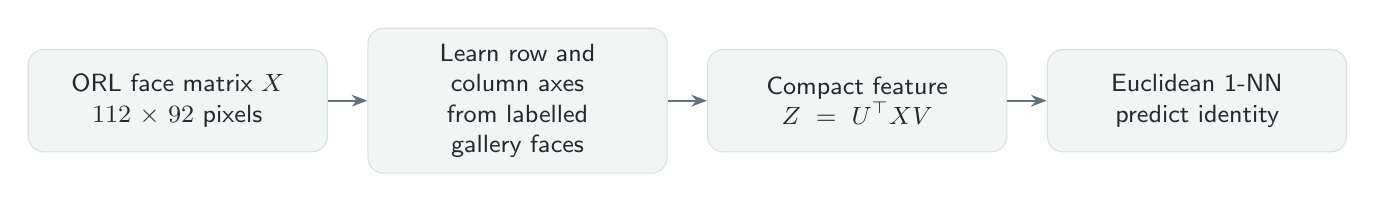
\begin{tikzpicture}[node distance=5mm]
  \node[stepbox] (x) {ORL face matrix $X$\\$112\times92$ pixels};
  \node[stepbox,right=of x] (learn) {Learn row and column axes\\from labelled gallery faces};
  \node[stepbox,right=of learn] (z) {Compact feature\\$Z=U^{\top}XV$};
  \node[stepbox,right=of z] (knn) {Euclidean 1-NN\\predict identity};
  \draw[arrow] (x)--(learn);
  \draw[arrow] (learn)--(z);
  \draw[arrow] (z)--(knn);
\end{tikzpicture}
\caption{Recognition pipeline. The learned projections are fitted on gallery images; probes are transformed only after fitting.}
\end{figure}

The discriminant tensor criterion (DTC) extends Fisher's between-class/within-class idea to projected matrices:
\[
J(U,V)=\frac{\displaystyle\sum_c n_c\left\|U^{\top}(\bar X_c-\bar X)V\right\|_F^2}
{\displaystyle\sum_c\sum_{i:y_i=c}\left\|U^{\top}(X_i-\bar X_c)V\right\|_F^2}.
\]
The numerator rewards separation between identity means; the denominator penalizes spread among images of the same identity. With one projection fixed, the other is updated by solving a generalized eigenproblem. MDA/2-1 learns one mode (the paper's 2-D LDA special case); MDA/2-2 alternates row and column updates. The final classifier is Euclidean one-nearest neighbour (1-NN), not part of the DTC optimization.

\begin{warmbox}
\smallcaps{Intuition}\quad Different people should land far apart; photos of the same person should stay compact. In our fixed MDA/2-2 setting, the learned 6\,$\times$\,6 feature has 36 values instead of the original 10,304 pixels.
\end{warmbox}

\begin{videobox}
\smallcaps{Project video}\par
\href{https://github.com/Lavalx100/comp3314-mda-face-recognition-replication/blob/main/output/video/Group27_MDA_Process_Explainer.mp4}{\sffamily\bfseries\color{Teal}Watch the 30-second MDA pipeline animation on GitHub}\par
{\sffamily\small\color{Muted}A landscape walk-through: gallery/probe split, projections, recognition, and results.}
\end{videobox}

\newpage
\section*{2 \; Data and experimental protocol}
We used the original Cambridge ORL database: 400 grayscale images of 40 identities, ten images per person, at 112 rows by 92 columns. Images were equalized independently. For each identity, 2, 3, 4, or 5 images formed the labelled \emph{gallery}; the remaining images were held-out \emph{probes}. Every method used the same deterministic split, and projections were fitted on gallery images only.

\begin{softbox}[left=1.5mm,right=1.5mm,top=1.2mm,bottom=1.2mm]
\begin{tabularx}{\linewidth}{>{\centering\arraybackslash}X>{\centering\arraybackslash}X>{\centering\arraybackslash}X>{\centering\arraybackslash}X}
{\displayfont\Large\color{Teal}400} & {\displayfont\Large\color{Teal}40} & {\displayfont\Large\color{Teal}10} & {\displayfont\Large\color{Rust}112\,$\times$\,92}\\
grayscale faces & identities & images per identity & pixels (rows $\times$ columns)
\end{tabularx}
\end{softbox}

The fixed-setting comparison averages 30 matched splits per gallery size: PCA with 36 components; Fisherfaces with full $N-C$ PCA pre-reduction and up to 36 LDA components; MDA/2-1 with six row components; and MDA/2-2 with 6\,$\times$\,6 components. All methods use Euclidean 1-NN. The dimension search uses five repeats. Choices needed because the paper is incomplete are: 64-level per-image histogram equalization, $\epsilon=10^{-4}$ with a 10-iteration cap, and a relative $10^{-6}$ ridge for singular within-class scatter. The seed rule is $3314+1000g+r$ for gallery size $g$ and repeat index $r$.

\smallcaps{Fixed-setting probe accuracy}\quad Mean $\pm$ sample standard deviation over 30 matched splits (percent).
\begin{center}
\scriptsize
\setlength{\tabcolsep}{4.1pt}
\begin{tabular}{lrrrr}
\toprule
Method & 2 gallery & 3 & 4 & 5\\
\midrule
Eigenfaces PCA & $73.9\pm2.5$ & $84.1\pm1.8$ & $88.2\pm3.0$ & $91.6\pm2.0$\\
Fisherfaces LDA & $73.1\pm2.8$ & $84.9\pm2.9$ & $88.0\pm2.4$ & $90.4\pm2.2$\\
\textbf{MDA/2-1} & $\mathbf{81.4\pm3.0}$ & $\mathbf{89.9\pm2.2}$ & $\mathbf{92.0\pm2.2}$ & $\mathbf{94.7\pm1.7}$\\
MDA/2-2, unit-L2 & $34.8\pm5.3$ & $52.6\pm5.6$ & $75.8\pm3.6$ & $87.5\pm2.8$\\
MDA/2-2, within-scatter & $5.4\pm1.9$ & $23.9\pm10.3$ & $64.0\pm6.0$ & $81.4\pm3.8$\\
\bottomrule
\end{tabular}
\end{center}

\begin{figure}[H]
\centering
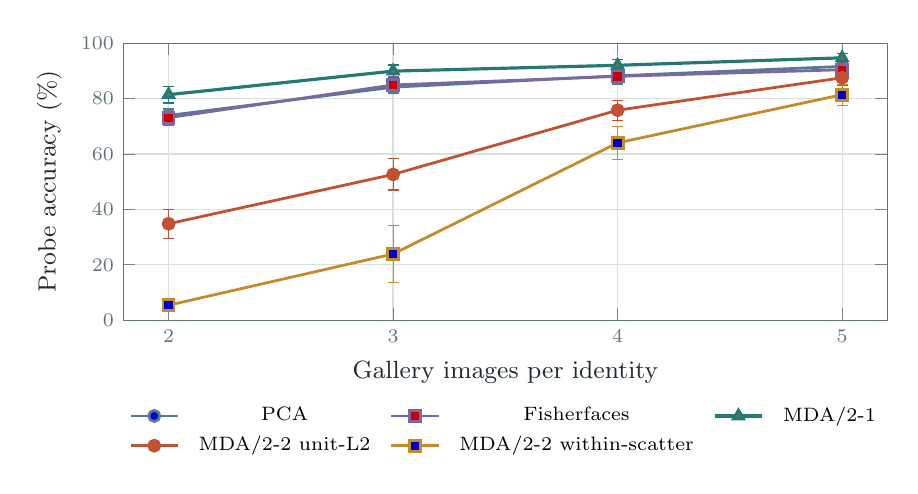
\begin{tikzpicture}
\begin{axis}[
  width=0.93\linewidth,height=5.1cm,
  xmin=1.8,xmax=5.2,ymin=0,ymax=100,
  xtick={2,3,4,5},ytick={0,20,40,60,80,100},
  xlabel={Gallery images per identity},ylabel={Probe accuracy (\%)},
  tick label style={font=\scriptsize,color=Muted},
  label style={font=\small,color=Ink},
  axis line style={color=Muted},
  grid=major,major grid style={draw=Rule,line width=0.45pt},
  legend style={draw=none,fill=none,font=\scriptsize,at={(0.5,-0.27)},anchor=north,legend columns=3,column sep=5pt},
  clip=false
]
\addplot+[color=Blue,mark=*,line width=1pt,error bars/.cd,y dir=both,y explicit] coordinates {(2,73.9) +- (0,2.5) (3,84.1) +- (0,1.8) (4,88.2) +- (0,3.0) (5,91.6) +- (0,2.0)};\addlegendentry{PCA}
\addplot+[color=Purple,mark=square*,line width=1pt,error bars/.cd,y dir=both,y explicit] coordinates {(2,73.1) +- (0,2.8) (3,84.9) +- (0,2.9) (4,88.0) +- (0,2.4) (5,90.4) +- (0,2.2)};\addlegendentry{Fisherfaces}
\addplot+[color=Teal,mark=triangle*,line width=1.15pt,error bars/.cd,y dir=both,y explicit] coordinates {(2,81.4) +- (0,3.0) (3,89.9) +- (0,2.2) (4,92.0) +- (0,2.2) (5,94.7) +- (0,1.7)};\addlegendentry{MDA/2-1}
\addplot+[color=Rust,mark=*,line width=1pt,error bars/.cd,y dir=both,y explicit] coordinates {(2,34.8) +- (0,5.3) (3,52.6) +- (0,5.6) (4,75.8) +- (0,3.6) (5,87.5) +- (0,2.8)};\addlegendentry{MDA/2-2 unit-L2}
\addplot+[color=Gold,mark=square*,line width=1pt,error bars/.cd,y dir=both,y explicit] coordinates {(2,5.4) +- (0,1.9) (3,23.9) +- (0,10.3) (4,64.0) +- (0,6.0) (5,81.4) +- (0,3.8)};\addlegendentry{MDA/2-2 within-scatter}
\end{axis}
\end{tikzpicture}
\caption{Fixed-setting results. Whiskers show sample standard deviation; MDA/2-1 is strongest at every gallery size.}
\end{figure}

\newpage
\section*{3 \; Full-grid evidence and critical interpretation}
For MDA/2-2, we evaluated all 10,130 feasible integer row/column dimension pairs, with five splits at each gallery size. That is 202,600 fits per normalization. The authors report their best MDA/2-2 Table I values across gallery sizes 2--5 as 90.1\%, 95.0\%, 98.3\%, and 99.0\% \cite{Yan2007MDA}.

\begin{figure}[H]
\centering
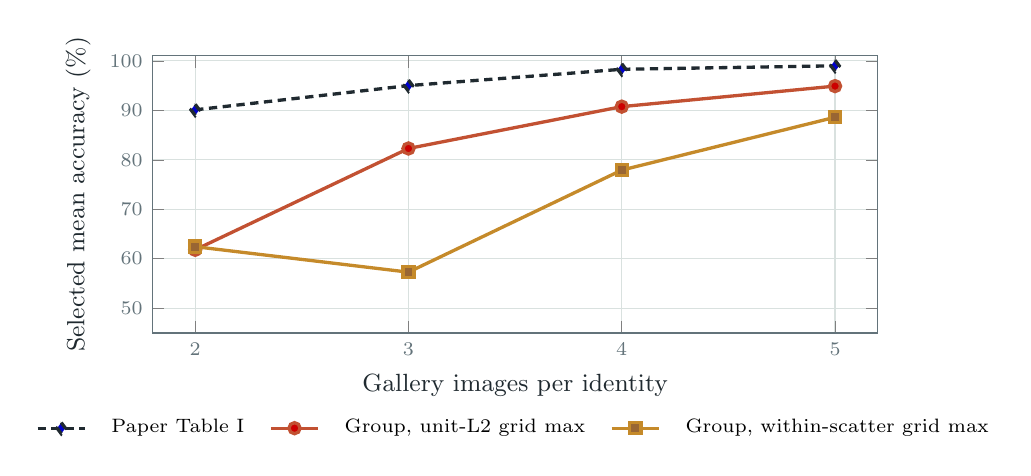
\begin{tikzpicture}
\begin{axis}[
  width=0.89\linewidth,height=5.1cm,
  xmin=1.8,xmax=5.2,ymin=45,ymax=101,
  xtick={2,3,4,5},ytick={50,60,70,80,90,100},
  xlabel={Gallery images per identity},ylabel={Selected mean accuracy (\%)},
  tick label style={font=\scriptsize,color=Muted},label style={font=\small,color=Ink},
  axis line style={color=Muted},grid=major,major grid style={draw=Rule,line width=0.45pt},
  legend style={draw=none,fill=none,font=\scriptsize,at={(0.5,-0.27)},anchor=north,legend columns=3,column sep=7pt},clip=false
]
\addplot+[color=Ink,mark=diamond*,line width=1.2pt,densely dashed] coordinates {(2,90.1)(3,95.0)(4,98.3)(5,99.0)};\addlegendentry{Paper Table I}
\addplot+[color=Rust,mark=*,line width=1.2pt] coordinates {(2,61.81)(3,82.29)(4,90.75)(5,94.90)};\addlegendentry{Group, unit-L2 grid max}
\addplot+[color=Gold,mark=square*,line width=1.2pt] coordinates {(2,62.44)(3,57.29)(4,77.92)(5,88.60)};\addlegendentry{Group, within-scatter grid max}
\end{axis}
\end{tikzpicture}
\caption{The group points are five-repeat dimension-search maxima. They are not unbiased test estimates and the paper's selection protocol is not fully reported.}
\end{figure}

The paper and group values are not a like-for-like comparison: the paper reports its best scores over dimensions, while our full-grid maxima use our own split and implementation choices. More importantly, our maximum dimension pair was selected using the same probe scores used to report that maximum. Projections were gallery-only, but this dimension-selection step reuses probe labels and makes selected peaks optimistic. A fairer estimate would choose dimensions using training-only validation and evaluate once on a separate outer test set.

\begin{softbox}
\smallcaps{The gallery-size-three dip}\quad The within-scatter grid maximum drops from 62.44\% at two gallery images to 57.29\% at three; the unit-L2 grid does not. In a separate 30-split nested-gallery diagnostic with dimension fixed at 6\,$\times$\,6, a third gallery image improves unit-L2 from 34.57\% to 53.05\% and within-scatter from 5.47\% to 26.70\%. The grid dip is therefore specific to the probe-selected within-scatter search, not evidence that more gallery images generally hurt.
\end{softbox}

\smallcaps{Strengths, limitations, and next step}\par\smallskip
\footnotesize
\begin{tabularx}{\linewidth}{@{}>{\raggedright\arraybackslash}X@{\hspace{4mm}}>{\raggedright\arraybackslash}X@{\hspace{4mm}}>{\raggedright\arraybackslash}X@{}}
\textbf{Strengths} & \textbf{Limitations} & \textbf{Best next experiment}\\[-1pt]
Original-resolution ORL; matched deterministic splits; full grids and assumptions documented. & Small, controlled dataset. The paper leaves seeds, scaling, equalization, singular-scatter handling, and selection details open. & Choose dimensions with gallery-only validation, test once on untouched data, then check another face dataset.\\
\end{tabularx}
\normalsize

\newpage
\section*{4 \; Efficient implementation and conclusions}
Exhaustive dimension search repeats many operations shared by nearby row/column sizes. The corrected optimized sweep caches class groupings and reuses generalized eigensystem factorizations, then forms each requested-size projection using the same shape-specific multiplication as a direct fit. This targets scatter construction and eigendecomposition without changing the mathematical objective or update order.

\begin{center}
\small
\begin{tabular}{lrr}
\toprule
Implementation (14 workers, one Accelerate thread) & Throughput & Peak memory\\
\midrule
Direct & 40.50 fits/s & 1.19 GiB\\
\textbf{Corrected cached (default)} & \textbf{47.48 fits/s} & \textbf{0.91 GiB}\\
\bottomrule
\end{tabular}
\end{center}

\smallcaps{Where the time goes}\quad Profile of 12 representative fits; most cost is in MDA fitting, not classification.
\begin{figure}[H]
\centering
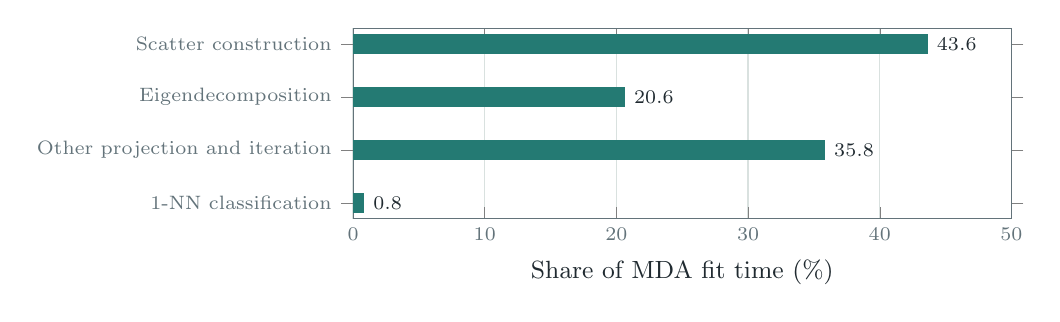
\begin{tikzpicture}
\begin{axis}[
  xbar,width=0.82\linewidth,height=4.0cm,
  xmin=0,xmax=50,
  ytick={4,3,2,1},
  yticklabels={Scatter construction,Eigendecomposition,Other projection and iteration,1-NN classification},
  xlabel={Share of MDA fit time (\%)},
  tick label style={font=\scriptsize,color=Muted},
  label style={font=\small,color=Ink},
  axis line style={color=Muted},
  xmajorgrids=true,major grid style={draw=Rule,line width=0.45pt},
  nodes near coords, nodes near coords align={horizontal},
  every node near coord/.append style={font=\scriptsize,color=Ink},
  bar width=7pt,
  clip=false
]
\addplot[fill=Teal,draw=Teal] coordinates {(43.6,4)(20.6,3)(35.8,2)(0.8,1)};
\end{axis}
\end{tikzpicture}
\caption{Stage profile from 12 representative direct fits. Classification is below 1\% of fit-plus-classification time.}
\end{figure}

The optimized path was about 17\% faster in the measured 60-fit benchmark and used 0.28 GiB less peak memory. A previous cache variant changed a few ill-conditioned gallery-size-2 fits; after correction, the 17 flagged settings matched the direct path under both normalizations for predictions, accuracy, iteration counts, sign-aligned projections, distances, and objectives. This is targeted validation, not an exhaustive pair-by-pair numerical comparison. The completed direct-run grids remain the canonical dataset; optimized code is the default for future sweeps.

\begin{warmbox}
\smallcaps{Runtime claim}\quad 71 minutes is an extrapolation from 47.48 fits/s to one 202,600-fit grid, not a completed optimized rerun. The original complete grids and all checkpoints are preserved; no exhaustive rerun was necessary.
\end{warmbox}

\section*{Conclusion}
On this fixed-setting ORL study, MDA/2-1 led the compared methods, while MDA/2-2 depended strongly on projection-axis normalization. The paper's best table was not numerically reproduced, and the available evidence does not isolate one cause: the article leaves several settings unspecified, and the group's grid maxima use probe data for dimension selection. The contribution is a transparent, original-resolution implementation, a complete preserved experimental record, and a faster path with targeted numerical checks—not a claim that MDA is universally superior.

\begin{softbox}
\smallcaps{Code and reproducibility}\par\smallskip
Source, run instructions, full grids, figures, and validation records:\par
\href{https://github.com/Lavalx100/comp3314-mda-face-recognition-replication}{\texttt{github.com/Lavalx100/comp3314-mda-face-recognition-replication}}.
\end{softbox}

\vspace{-1mm}
\begin{thebibliography}{9}
\setlength{\itemsep}{0.1em}
\small
\bibitem{Yan2007MDA} S. Yan, D. Xu, Q. Yang, L. Zhang, X. Tang, and H.-J. Zhang. Multilinear discriminant analysis for face recognition. \emph{IEEE Transactions on Image Processing}, 16(1):212--220, 2007. doi: \href{https://doi.org/10.1109/TIP.2006.884929}{10.1109/TIP.2006.884929}.
\bibitem{ORL} AT\&T Laboratories Cambridge. The Database of Faces (ORL), 1992--1994. \url{https://cam-orl.co.uk/facedatabase.html}.
\end{thebibliography}

\end{document}
